\documentclass{article}
\usepackage[frenchb]{babel}
\usepackage[utf8]{inputenc}
\usepackage[T1]{fontenc}
\usepackage{amsthm}
\usepackage{algpseudocode}
\usepackage{graphicx}
\algrenewcommand\algorithmicif{\textbf{Si}}
\algrenewcommand\algorithmicdo{\textbf{Faire}}
\algrenewcommand\algorithmicfor{\textbf{Pour}}
\algrenewcommand\algorithmicwhile{\textbf{Tant que}}
\algrenewcommand\algorithmicend{\textbf{Fin}}
\algrenewcommand\algorithmicelse{\textbf{Sinon}}
\algrenewcommand\algorithmicthen{\textbf{Alors}}
\newtheorem*{prop}{Propriété}
%Faudrait aller à la ligne après le titre de la ppté/déf avant d'écrire la déf/prop, non ?
%J'ai pas compris
\newtheorem*{ddef}{Définition}
\newtheorem{tth}{Théorème}
\title{Projet 1 (C) : Voyageur de commerce}
\author{Alexandre Talon \& Grégoire Beaudoire}
\begin{document}
\maketitle
\tableofcontents
\section*{Introduction}
On a ici réalisé un projet de programmation dans le langage C. Ce projet, qui a duré sept semaines, a été en grande partie réalisée en monôme par Alexandre Talon, avec une participation tardive de Grégoire Beaudoire.

On étudie le problème problème d'optimisation classique du voyageur de commerce : il s'agit de parcourir une liste de ville donnée et de revenir à la ville de départ
en un chemin de longueur minimale. D'un point de vue plus formel, on peut voir les villes comme étant les sommets d'un graphe, la distance entre deux villes le poids de 
l'arête reliant les sommets correspondant, le problème étant de trouver un cycle hamiltonien de longueur minimale.


Il s'agit en fait d'un problème NP-complet, c'est-à-dire qu'on ne dispose pas d'algorithme le résolvant de manière exacte en un tems polynomial en fonction de la taille
de l'entrée (villes et distances entre chaque paire de villes). On s'intéresse alors à un algorithme résolvant le problème du voyageur de commerce de manière approchée :
on cherche à programmer un algorithme permettant de trouver une tournée passant par toutes les villes imposées par l'utilisateur, le tout en un temps raisonnable et en
fournissant une réponse pas trop éloignée de la réponse optimale.
%note : il faudrait reformuler ce paragraphe, les formules utilisées ressemblent trop au sujet du projet.


Pour y parvenir, il est nécessaire de choisir des structures de données adaptées aux données que l'on va stocker et à la façon dont on les utilise. On cherche
ici à optimiser le temps mis à l'exécution des divers algorithmes, tout en limitant raisonnablement la place occupée par les données en mémoire. On commencera par
décrire ces structures et la façon dont elles sont implémentées. Dans un second temps il sera question des algorithmes à proprement parler utilisés pour résoudre
le problème. On terminera par le choix de l'interface utilisateur.

\section{Structures de données}

On utilise dans ce projet deux structures non triviales : d'une part des tas, d'autre part des arbres arbres binaires de recherche équilibrés de type arbres AVL.
\subsection{Tas}

Un tas est un arbre binaire complet vérifiant la propriété suivante : l'étiquette de tout noeud différent de la racine est supérieure à l'étiquette de son père.
De plus, l'arbre est rempli \og dans l'ordre \fg : si $h$ est la profondeur de l'arbre, alors tous les étages de profondeur plus petite que $h$ sont remplis.

D'un point de vue pratique, on peut stocker cet arbre binaire dans un tableau $t$. Pour des raisons pratiques, on place la racine en $t[1]$. Alors si un noeud est
en position $i$, donc dans $t[i]$ alors son fils gauche est dans $t[2*i]$ et son fils droit dans $t[2*i+1]$. De plus le père de $t[i]$ est en $t[E(i/2)]$, où $E(x)$
désigne la partie entière de $x$. On peut ainsi calculer très facilement les positions des fils et du père d'un noeud.

Aussi, dans ce projet on a besoin de tas dont on connaît la taille maximale, on ne change donc pas la taille du tableau utilisé pour stocker le tas au fur et à mesure
de son utilisation.

Cette structure supporte plusieurs opérations, décrites ci-dessous.

\subsubsection{Accès au plus petit élément}
Il est trivial d'accéder au plus petit élément d'un ensemble stocké dans un tas : il s'agit de l'étiquette de la racine. Ceci découle immédiatement de la propriété
d'ordonnancement des noeuds.


\subsubsection{Insertion}
Lorsqu'on ajoute un élément, on ne peut se contenter de l'ajouter à la première case libre car alors la propriété sur les étiquettes des arbres ne serait plus respectée.
Pour insérer un élément, on procède donc comme suit. On commence par ajouter l'élément à la première place libre. Puis tant que l'étiquette de ce noeud est plus 
petite que celle de son père on échange ces deux noeuds de place, et on continue avec le même noeud. Dans notre cas, il faut vérifier que l'on s'arrête une fois que
le noeud est devenu la racine. On gère ce problème en posant $t[0] = -1$. Comme toutes les étiquettes sont positives, ceci agit comme une barrière.

\subsubsection{Suppression de la racine}
Dans un tas on ne s'autorise la suppression que de la racine, donc du minimum du tas. Il faut alors trouver une nouvelle racine. On commence par choisir le noeud le 
dernier noeud de l'arbre comme racine. Ceci permet de conserver la propriété de complétude du tas. Ensuite, on fait descendre ce noeud dans l'arbre : tant que ce noeud
est plus grand que le plus petit de ses fils, on échange ces deux noeuds et on continue avec le même noeud. La complétude de l'arbre est donc bien conservée.

\subsubsection{Performances}
Notons tout d'abord $h$ la hauteur de l'arbre binaire, et $n$ le nombre de noeuds qu'il contient. Comme cet arbre est binaire et complet, on a $h = E(log(n))$.
%fin environ, à affiner...
La lecture du plus petit élément du tas se fait en $O(1)$.
L'insertion et la délétion, correspondant à un parcours dans l'arbre, sont donc en $O(h) = O(log(n))$.
Enfin, un tas prend $O(n)$ en mémoire.


Ces propriétés font du tas une structure utile pour maintenir le minimum d'un ensemble auquel on ajoute des éléments et retire le minimum. Il est utile, comme nous le
verrons ci-dessous, pour l'algorithme de Prim.

\subsection{Arbres AVL}

Commençons par définir les arbres binaires de recherche :
\begin{ddef}[ABR]
Un arbre binaire de recherche, ou ABR, est un arbre où chaque noeud possède une étiquette telle que, en notant $(gc, x, dr)$ un noeud, où g est le sous-arbre gauche, $x$ l'étiquette et dr le sous-arbre droit : pour tout noeud $N = (gc^{\prime},y,dr^{\prime}) \in gc$, $y < x$, et
pour tout noeud $N^{\prime}=(gc^{\prime\prime},z,dr^{\prime\prime}) \in dr$, $z > x$.
\end{ddef}

Les arbres AVL sont des arbres binaires de recherche. Ils présentent en outre la particularité d'être automatiquement équilibrés, c'est-à-dire :

\begin{ddef}[Arbre équilibré]
Un arbre équilibré est un arbre dans lequel la hauteur des deux sous-arbres de tout noeud diffère d'au plus un.
\end{ddef}

Pour pouvoir définir plus aisément la notion de "différence de hauteur de sous-arbre", on va définir le facteur d'équilibrage :

\begin{ddef}[Facteur d'équilibrage d'un noeud]
Le facteur d'équilibrage d'un noeud est la différence entre la hauteur de son sous-arbre droit et celle de son sous-arbre gauche.
\end{ddef}

Ainsi un arbre équilibré est simplement un arbre dont le facteur d'équilibrage de tout noeud est compris entre $-1$ et $1$. Nous allons commencer par voir les opérations basiques qu'on peut effectuer sur ces arbres, puis nous verrons comment rééquilibrer un arbre.

\subsubsection{Opérations basiques}

Nous allons ici voir les opérations de base, \textit{ie} l'insertion et la suppression.

D'abord, l'insertion : pour insérer un élément $x$ dans un arbre binaire de recherche, équilibré ou non, on va parcourir l'arbre pour trouver sa place. Ainsi l'algorithme peut s'écrire :

\begin{algorithmic}
\If{L'arbre est vide}

Créer l'arbre réduit à l'élément que l'on veut insérer

\ElsIf{$x >$ étiquette de la racine}

Insérer x dans le sous-arbre droit

\Else

Insérer x dans le sous-arbre gauche
\EndIf
\end{algorithmic}
On peut évidemment obtenir des arbres déséquilibrés après une insertion, on expliquera plus tard sur la manière d'équilibrer un arbre. Il est en revanche clair qu'on a toujours un arbre binaire de recherche après l'insertion.
%clair ?

La suppression maintenant : on a plusieurs cas, suivant si le noeud à supprimer possède des fils ou pas :

\begin{algorithmic}
\If{Le noeud n'a pas de fils}

Supprimer le noeud

\ElsIf{Le noeud a un fils}

Supprimer le noeud et le remplacer par son fils

\Else

Supprimer le noeud, le remplacer par son successeur, \textit{ie} l'élément le plus à gauche dans son sous-arbre droit.
\EndIf
\end{algorithmic}
Si le noeud n'a pas de fils ou un seul fils, on garde trivialement la structure d'arbre. S'il en a deux, comme on le remplace par le plus petit élement plus grand que lui, on garde la structure d'arbre : les éléments du sous-arbre gauche sont toujours plus petits que cette nouvelle racine, et tous les éléments du sous-arbre droit étaient plus grands que leur plus petit élément, ils sont donc plus grand que cette nouvelle racine.

Ces opérations basiques sont valables pour les arbres binaires de recherche en général cependant. Les arbres AVL s'utilisent comme les arbres binaires de recherche, mais on peut également effectuer sur eux les opérations de rééquilibrage. Pour rééquilibrer 
un arbre déséquilibré, on effectue ce qu'on appelle des rotations. Il convient tout d'abord de remarquer qu'un noeud peut être déséquilibré de deux façons : il peut 
être "left heavy", c'est-à-dire qu'il possède un facteur d'équilibrage inférieur ou égal à $-2$, ou "right heavy", c'est-à-dire qu'il possède un facteur 
d'équilibrage supérieur ou égal à $2$. Nous allons commencer par voir comment résoudre ces problèmes par des rotations simples, puis remarquer qu'elles ne suffisent pas 
dans certains cas où il est obligatoire d'utiliser des rotations doubles.

\subsubsection{Rotations simples}
Considérons l'exemple intuitif de déséquilibrage, qu'on pourrait représenter sous la forme (vide, x, (vide, y, (vide, z, vide))) : un noeud x possédant un fils droit y et pas de fils gauche, et y possédant un fils droit z et pas de fils gauche. Cet arbre est déséquilibré : en effet son facteur d'équilibrage vaut $2$, la hauteur de son sous-arbre droit étant $2$ et celle de son sous-arbre gauche $0$. Pour l'équilibrer, on va effectuer une rotation :

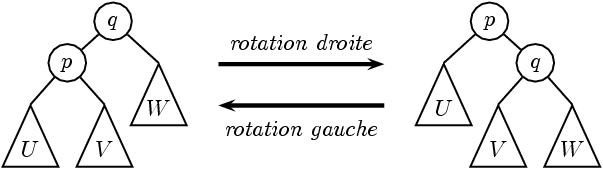
\includegraphics[width = 10cm]{poly093.jpg}

Ainsi on peut résoudre notre problème d'arbre déséquilibré en faisant une simple rotation gauche. Cependant, les simples rotations ne permettent pas de conclure dans tous les cas. Des problèmes vont apparaître lorsque un arbre et son sous-arbre dominant ne \guillemotleft penchent \guillemotright\ pas du même côté : quand on a un arbre right heavy, avec un sous-arbre droit right heavy, ou un arbre left heavy, avec un sous-arbre gauche left-heavy, on peut appliquer une simple rotation. Quand on a un arbre right heavy avec un sous-arbre droit left heavy, et inversement, les rotations simples ne donnent rien.
%clumsy

Ainsi les rotations simples ne suffisent pas pour rééquilibrer tous les abres : il est nécessaire d'utiliser ce qu'on appelle des rotations doubles pour pouvoir avoir un algorithme général de rééquilibrage.
%Détailler un peu, c'est très concis, probablement trop.

\subsubsection{Rotations doubles}
L'idée des rotations doubles est de d'abord travailler sur le sous-arbre, pour se ramener à un cas simple \guillemotleft droit\guillemotright\ qu'on peut résoudre avec une rotation simple. Les rotations doubles fonctionnent comme suit :

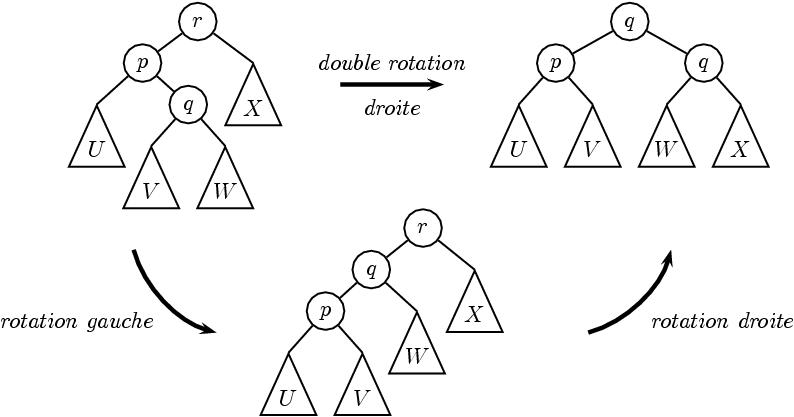
\includegraphics[width = 10cm]{poly095.jpg}

Ainsi, avec les simples rotations et les doubles rotations, on peut maintenant équilibrer tous les arbres déséquilibrés et ainsi garantir cette propriété d'équilibrage.

\subsubsection{Algorithme d'équilibrage}
Lors d'insertions ou délétions, il peut arriver que l'on obtienne un arbre déséquilibré. Dès qu'on rencontre un n\oe ud ayant un "<mauvais"> facteur d'équilibrage,
on applique un rééquilibrage, dont le pseudo-code est ci-dessous.

\begin{algorithmic}
\If {L'arbre est right heavy}

\If {Le sous-arbre droit de la racine est left heavy}

Effectuer une double rotation gauche.
\Else

Effectuer une simple rotation gauche.

\EndIf
\ElsIf {L'arbre est left heavy}

\If {Le sous-arbre gauche de la racine est right heavy}

Effectuer une double rotation droite.
\Else

Effectuer une simple rotation droite.
\EndIf
\Else

Ne rien faire : l'arbre est équilibré.
\EndIf
\end{algorithmic}




\section{Algorithme de Prim}
Le but de l'algorithme de Prim est de renvoyer un arbre couvrant minimal d'un graphe connexe donné en entrée.

D'abord, il convient de se demander ce que fait réellement cet algorithme. Pour comprendre ce qu'il se passe, nous allons avoir besoin de quelques définitions :

\begin{ddef}(Arbre couvrant minimal)
 Un arbre couvrant est un ensemble d'arêtes tel qu'entre toute paire de sommets du graphe il existe un chemin les reliant et n'empreintant que des arêtes de cet
 ensemble.
 On dit de plus qu'un arbre couvrant est minimal si la somme des poids de ses arêtes est inférieure à la somme des poids des arêtes de tout autre arbre couvrant.
\end{ddef}

\subsection{Algorithme}

\subsection{Implémentation}

\section{Algorithme TSP}
On utilise au c\oe ur de ce projet l'algorithme TSP qui, comme précisé dans l'introduction, donne une réponse approchée au problème du voyageur de commerce.

\subsection{Algorithme}
L'algorithme TSP est en fait assez simple. Il s'agit tout d'abord d'obtenir un arbre couvrant minimal du graphe considéré.


On construit, dans ce projet, cet arbre couvrant à l'aide de l'algorithme de Prim décrit ci-après.

Une fois que l'on a un arbre couvrant minimal, l'algorithme TSP consiste à partir d'un sommet et parcourir l'arbre en conservant les sommets rencontrés dans l'ordre où 
on les a rencontrés dans l'arbre. On ne garde alors que la première occurence de chaque sommet et on renote le premier sommet à la fin (on doit revenir au point de 
départ). La réponse de l'algorithme est alors cette liste de villes.

\subsection{Implémentation}
L'algorithme de Prim que l'on a codé nous renvoie un arbre couvrant minimal sous la forme d'une liste d'adjacence : il s'agit d'un tableau $adj$ tel que
$adj[i]$ contienne la liste des voisins de $i$ dans l'arbre.
On effectue alors un parcours infixe
%c'est bien ça, non ?
des sommets de cet arbre. Afin de ne pas voir des sommets plusieurs fois, on déclare un tableau $seen$ dont la $i$-ème case vaut $true$ si et seulement si on a déjà
visité le sommet $i$ au cours du parcours. On note donc dans un tableau le sommet en cours de visite, on le marque comme déjà vu, puis on visite récursivement ses 
fils non encore visités. On leur indique à partir de quelle case du tableau écrire les villes que cette visite parcourera. Puis quand on passe au voisin suivant, on a
récupéré l'adresse de la case du tableau à laquelle l'écrire, et ainsi de suite.

%idée : si la première ville n'est pas fixée, on peut essayer en partant de chaque ville et voir la distance minimale obtenue ? est-ce que ça diffère selon la ville 
%choisie ? (je pense que oui)


\section{Utilisation}

\subsection{Interface utilisateur; compilation}
%wtf titre
%Comment l'algorithme fonctionne et réagit à l'utilisateur.

\subsection{Complexité}

\section*{Conclusion}



%BIBLIOGRAPHIE





\end{document}
